\chapter{Analysis}\label{chap:analysis}
Before being able to design a solution to above mentioned problem, a more detailed description of the said problem, along with the wishes and limitations established by Zoo, is needed. 

\section{Implicit Human Computer Interaction}

%conc
The thought between implicit interaction is that the same subtle principles that governs interaction between people also controls the interactions with computers \cite{Schmidt2000}. " sensing
and computation need to be augmented with an understanding of the unstated expectations we
people have from our interactive counterparts"

By using how people achieve various interaction goals between each other one could isolate these interactions and apply to Human Computer Interaction (HCI)

Reeves and Nass coined the Media Equation which states that \cite{mediaequation} interactive objects are engaged with as if they were real people. This ties together with implicit interaction as this is based on these interactions. Furthermore, the last of the eight media equation propositions states that people already know how to behave in the real world and therefore this can be translated to computer interaction.

This should be considered when creating a prototype.

%Implicit human computer interaction is important to consider as it differentiates itself from explicit human computer interaction which encompasses more traditional interactions where the user directly expects a reaction from their initial action.

\section{Problem area}
A meeting with Zoo was held, to get an elaboration and clarification on Zoo's challenges, limitations, needs and wishes, and to exchange ideas for possible solutions. During the meeting, it became clear that an important aspect of the project, would be to maintain the spirit of Zoo, by staying true to the nature of the animals, and creating a family friendly, informative, experience based around the animals.
From this, a descriptive guideline for the project, based on the needs and wishes of Zoo was created:  

\begin{itemize}
    \item[-] The installation should add some degree of value to the user, in terms of an experience. 
    \item[-] The experience must concern the animals located in same area as the installation, to achieve a coherent experience.
    \item [-] The experience should be informative\todo{Not a direct necessary requirement}.
    \item[-] If animals are to be represented, it must be done in respect to the natural behavior of the animal. An example of a violation of this would be to humanize the animals by, for instance, animating talking animals. 
    \item[-] The experience should not be age specific, but should preferably primarily appeal to children, and secondarily their parents, as this target group is the most represented audience in the park. 
    \item[-] The interaction level should be simple and straightforward, and shouldn't need more than the users themselves to be able to perform the interactions. Therefore no controllers or wearables must be used. 
    \item[-] The experience should preferably not be dependent on the season, but instead encourage all-year-use . As so, it was suggested to make an experience that could be used in weather conditions where most animals will not be outdoors for the guest to see.
    \item[-] During a guest's visit, the installation should strive to occupy them, with an entertaining experience, such that the entire park is less likely to be explored in one trip. Making a guest more likely to return in the future.
\end{itemize}

    % Baseret på dyr, relevant for omgivelser
    % Saglig, ikke fjollet
    % Informativt
    % Børnehøjde men OGSÅ til voksne!
    % Simple interaktion, ingen controllerer.
   
    % Ikke bundet til en specifik sæson.
    % Gæster skal gå derfra med en oplevelse/ værditilførelse.
    % Design skal gerne kunne holde på folk.

% examples of existing installations in the park.


% possible locations
% statistics about the target group (børn og voksne) 

% FPS 





% NEW SECTION! 
% How to design to both children and adults 
% interactive displays 
% Sota for both hardware and software, projects mm. - SKAL sættes i perspektiv med interviewets fund! - bruges som design inspiration. 

% Design requirements ( based on all the things above) 




\section{Perception}
"Perception is the ability to become aware of something through human senses (hearing, seeing, feeling etc)\\

% https://ieeexplore.ieee.org/document/1667620/#full-text-section

% https://link.springer.com/article/10.1007/BF00896880

% file:///Users/damh/Downloads/927-3572-1-SM.pdf

% http://diposit.ub.edu/dspace/bitstream/2445/49643/1/631349.pdf

% https://www.interaction-design.org/literature/topics/visual-hierarchy

% https://dzone.com/articles/visual-perception-and-its-influence-in-ux-design-1

\section{The seven stages of action} % Simon
    The seven stages are awesomegaysauce. 



\section{Interactive public displays} % Daniel
    Interactive public displays are different from an interaction perspective than the normal use of displays that a user might be used to\cite{interactivePublicDisplays}. Mostly this difference comes from the interaction not beginning directly from interacting with the display, but happens in more indirect sense. To better understand why this is, the interaction phases of an interactive public display has been broken down into 6 different stages, as seen in \autoref{fig:audienceFunnel}. A user only goes between phases, when passing a threshold, e.g. for a user to pass into the first phase, their attention must be caught\cite{interactivePublicDisplays}.
    
    \begin{figure}[H]
    	\centering
    	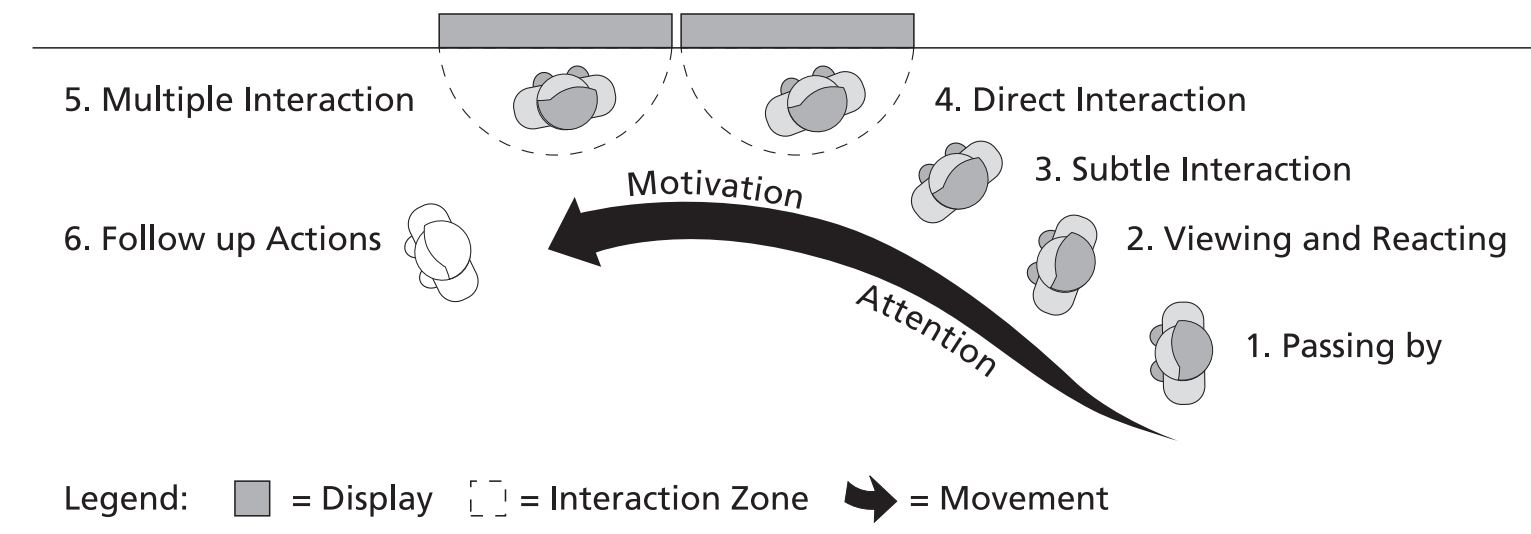
\includegraphics[width=0.9\linewidth]{figure/Analysis/AudienceFunnel.png}
    	\caption{The interaction phases of an interactive public display being broken down into 6 stages, compiled into the audience funnel model\cite{interactivePublicDisplays}.}
    	\label{fig:audienceFunnel}
    \end{figure}
    
    The entire interaction with the display only starts when a potential user gets their attention caught by the display. The attention grabbing mechanism of the display can vary wildly in implementation and style, but can in general terms be broken down into bottom-up processes and top-down processes\cite{interactivePublicDisplays}. Bottom-up processes involve some external stimuli that via something unexpected can help grab attention from a user, these can be a suddenly appearing polar bear, an error message, or any other item that the user might not have been looking for\cite{interactivePublicDisplays}. Top-down processes revolve around a user having a form of a goal that will guide their attention towards what they are looking for\cite{interactivePublicDisplays}, e.g. if a user was looking for a penguin, and a penguin was observed in their vision, their attention would be guided towards it.
    
    The second phase is entered after the user has become aware of the existence of the display, and might have turned their head, diverted their gaze towards the display or performed any action as an effect of the display\cite{interactivePublicDisplays}.
    
    While in the beginning of the interaction with the display, it is mostly reliant on attention from the user, but when a user is in the third phase, it becomes more dependent on the motivation to interact\cite{interactivePublicDisplays}. This motivation can be increased using curiosity and exploration\cite{interactivePublicDisplays}. Curiosity, according to the article, is described as 
    \begin{quote}
        \textit{"a precursor to explorative behavior, through which people make accessible previously unavailable information about their environment."}\cite{interactivePublicDisplays}
    \end{quote}
    So by presenting some information and leaving out some gaps, or having a puzzle missing one more piece to be finished, the user might become curious and start exploring the possibilities of e.g. putting in the last the piece of said puzzle\cite{interactivePublicDisplays}.
    
    The third phase begins when what was displayed during the second phase, makes the user curious enough to physically divert their body towards the display, or making any movement that is meant to cause the display to react, while not necessarily being in frame of the screen. At this point, it is the goal that the user's motivation to interact is high enough to enter the next phase, direct interaction\cite{interactivePublicDisplays}.
    
    The fourth phase of direct interaction is when a user has either positioned themselves in front of the display, or simply has entered the interaction zone of the display. In the case of the Magical Mirrors mentioned in the article\cite{interactivePublicDisplays}, the interaction zone, was the right dashed circle displayed in \autoref{fig:audienceFunnel}, while the left dashed circle was a secondary scree, that might be used when in phase five; Multiple interaction.
    
    The fifth phase of the interaction is started when a user, in the case of the magical mirrors, either goes from one display to another, or comes back for another interaction after ending the first\cite{interactivePublicDisplays}.
    
    The sixth and final phase the interaction might end with, is the follow up phase, where a user might do an action following up the interaction from the display. This might entail using their smartphone, to search for more information about the display or information gotten from the display during the interaction, or take a photograph of themselves or their friends still doing interaction\cite{interactivePublicDisplays}. 
    
    \subsection*{Conclusion}
        The audience funnel describes the different phases of interaction a user might have with an interactive public display. A user won't necessarily follow the phases linearly, but might jump past direct interaction, and instead take pictures of their friends directly interacting with the display. The attention grabbing mechanics that are supposed to entice a user to enter the second and third phase, are discussed more in detail in \autoref{sec:visualAttention}.
\section{Invoking action in users} % Søren
%seven stages of action \cite{DesignOfEverydayThings} \cite{Norman1983}

\cite{interactivePublicDisplaysKinect}

\section{Visual attention}\label{sec:visualAttention}

In "What attributes guide the deployment of visual attention and how do they do it?" Jeremy. M Wolfe explores which attributes guide visual attention\cite{Wolfe2004}.

For this an example image is shown
\begin{figure}[H]
    	\centering
    	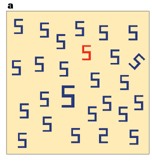
\includegraphics[width=0.4\linewidth]{figure/Analysis/natureFig1.png}
    	\caption{The red, the tilted or the big 5 are easy to find, the 2 not so much\cite{Wolfe2004}.}
    	\label{fig:hard2find}
    \end{figure}

Based on several features like the ones in the picture, tests were conducted to rank the time and efficiency with which they were isolated. The study resulted in a table of attributes that could guide attention

\begin{figure}[H]
    	\centering
    	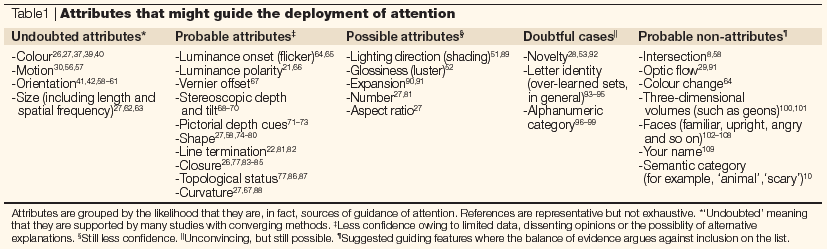
\includegraphics[width=0.9\linewidth]{figure/Analysis/attributes2find.png}
    	\caption{List of attributes and their importance\cite{Wolfe2004}.}
    	\label{fig:attributes2find}
    \end{figure}
\todo{MAKE OWN TABLE}
Considerations to include, if possible, all undoubted attributes as well as some probable attributes that guides attention should be made in the creation and installation of a display. All of these features are put into effect if they are different relative to their environment. As example if a display were of different luminance to it surroundings, it would probably attract attention.

\section{Gamification}
    The definition of gamification this report is adhering to, is defined by Sebastian Deterdin et al as being: \begin{quote}
        \textit{"the use of game design elements in non-game contexts"}\cite{gamification}.
    \end{quote}
    The paper tries to define gamification due to the popularity the word has gotten in both the industry and scientific space\cite{gamification}\todo{Hvad er formålet med denne sætning?}. According to another paper by Karl Kapp\cite{gamificationMyths}, there are four myths about the umbrella term \textit{gamification}\cite{gamificationMyths}. Of the four, two are the most relevant for this paper \todo{gennemgå afsnittet og konstater at alle "papers" mener artikler, og ikke vores raport}. The first myth, is that gamified interactions and games are the same, which isn't true\cite{gamificationMyths}. Games have a decided end and start, while interaction based gamification don't necessarily have such start and finish\cite{gamificationMyths}. In games, the player usually have some expectation of a goal or win condition, while the same can't necessarily be said for a gamified interaction\cite{gamificationMyths}. The other myth is that gamification is all about points and achievements and rewards, and while these can play apart of a gamified experience, most games have much more than this\cite{gamificationMyths}. According to the paper, most games also have elements of story, challenge, continual feedback and a high level of interactivity, something that a gamified interaction doesn't have\cite{gamificationMyths}.\\
    
    An example of gamification is Khan Academy\footnote{Khan Academy: \url{https://www.khanacademy.org/}}. The website is used for learning various subjects, like mathematics, electrical engineering or Physics, and tries to emphasize learning using a point system, streak counter for right answers and progress tracking per subject basis\cite{khanacademyGamfication}. This is a very rudimentary implementation of gamification, but it serves its purpose of motivating a user to learn\cite{khanacademyGamfication}.
    
\section{Zoo Tech}
Interactive technology and human–animal encounters at the zoo - https://www.sciencedirect.com/science/article/pii/S1071581916300477

"Firstly, interactive technology at the zoo risks distracting from visitors' encounters with animals.

Secondly, the appearance and use of technology moreover runs counter to expectations of naturalistic zoo landscapes. 

Thirdly, interactive systems however offer opportunities to enhance important aspects of visitors' experience of animal encounters, and to widen the temporal and spatial dimensions of the encounter. 

Finally, we interpret these insights by examining how technology is used in the context of interactions between numerous human and animal actors, and in a setting impacted by complex social and organizational forces."

https://www.youtube.com/watch?v=XxTQOD9NI5g

\section{Designing engaging experiences for children and their parents}
\todo{This section doesn't have to be its own section. There are some aspects of target group analysis and later some designing for children}
Since a zoo is predominantly a place for families with children (Between 60 to 80\% worldwide)\cite{togetherAtTheZoo} it is relevant to study their shared experience in order to design engaging interactive installations aimed at children without neglecting the parents.
A theoretical framework based on existing literature suggests that \textit{social bonding} with their children is considered the primary experience from the parents' perspective, with \textit{"edutainment"}\footnote{Entertainment that is designed to be educational. Meriam-webster's definition can be seen here: \url{https://www.merriam-webster.com/dictionary/edutainment}} being a secondary goal of a visit at the zoo. Parents are interested in providing learning experiences for their children. However, \textit{entertainment} is the primary goal and \textit{togetherness} the secondary for children\cite{togetherAtTheZoo}. The learning aspect is not a priority for the younger children, at least not during the entire visit. Older children tend to have more curiosity towards detailed knowledge about the animals and read from the information boards together with their parents\cite{togetherAtTheZoo}. Through interviews with families conducted in Aalborg Zoo it was found that, aside from activities involving animals, physical activities in the zoo playground are also central for children when visiting the zoo. The occasional break from passively watching the animals, by partaking in physical activities, helps the children refocus when returning to explore the animals\cite{togetherAtTheZoo}.

Digital technology is used more and more in zoos today in order to make the zoo experience increasingly engaging and educational through interactivity\cite{webberInteractiveTechInZoo}. It has the potential to be a very effective delivery system of information and raises awareness of e.g. conservation issues or animal welfare. Furthermore, it can create learning experiences that are attractive to children as well\cite{webberInteractiveTechInZoo}. The challenge of designing such interactive systems, however, is to design it in such a way that it enhances the human-animal encounters without stealing focus from it\cite{webberInteractiveTechInZoo}. A study shows that, instead of reading information of a sign, using live or video presentations helps visitors gain more knowledge about a zoo exhibit and makes them stay at the exhibit longer\cite{presentationStayDuration}.

When designing an interactive public display or art installation ease-of-use is often considered the main goal of the user experience\cite{Hull2018}. The following experience model is based on an idea workshop with soundscape artists and children and it illustrates what aspects are also important to children when it comes to interactive experiences (See \autoref{fig:provisionalModelOfConsumerExperience}). Challenges in creativity and physical and mental skills are a priority. As is socializing or competing with others and also some form of sensation, such as touch, smell, taste etc. and having to use their imagination in some way.
\todo{Create a new "provisional model of consumer experience" from the article}
\begin{figure}[H]
    	\centering
    	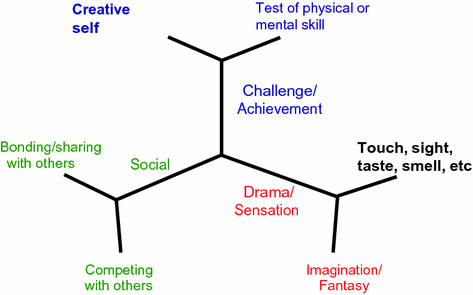
\includegraphics[width=0.9\linewidth]{figure/Analysis/provModelExp.png}
    	\caption{Provisional Model Of Consumer Experience\cite{Hull2018}}
    	\label{fig:provisionalModelOfConsumerExperience}
\end{figure}

\subsection{Sub conlusion}
Other than social bonding, educating children is a priority for parents when bringing their children to the zoo. It is not, however, a priority for the children who tend to lose focus from watching animals for too long\cite{togetherAtTheZoo}. Interactive digital technology can be used to enhance children's interest in learning about animals\cite{webberInteractiveTechInZoo}. When designing such interactive systems three aspects of interactive experiences(Challenge, Social, Sensation) should be kept in mind\cite{Hull2018}.

\section{Designing for children}
When considering Zoo's population of visitors, a vast majority of the visitors are children of different ages(insert data from zoo when we get it here). Therefore, it is important to research and understand how to design for children as in comparison to adults. 
When designing for children, cognitive and physical development is an important matter to be considered\cite{kidsDesign}. Furthermore, the role of the family is also an important aspect when it comes to how the children perceive the digital experience\cite{kidsDesign}.

\subsection{Design principles}
When discussing design principles with the focus on children, a list of compiled principles have been made by the children's design guide\cite{kidsDesign}, which consists of a team of 70+ 'heroes' which comes from different backgrounds such as designers, psychologist and neuroscientists. The ten principles can be seen in \autoref{princelist}.

\begin{enumerate}\label{princelist}
    \item \textbf{Everyone can play} I need a product that does not discriminate against characteristics such as gender, age, ability, language, ethnicity, and socio-economic status.
    \item \textbf{Give me control and offer support} Give me the tools I need to adapt to your product or service. Consider where i am in my development to both inspire me and nurture my growth.
    \item \textbf{I have purpose so make my influence matter} Help me understand my place and value in the world.
    \item \textbf{Offer me something safe} Ensure you provide me with a model for healthy behaviour, and do not forget that my data should be handled with utmost respect and care.
    \item \textbf{Create space for play (including a choice to chill)} When using your product or service, consider different moods, view and contexts of play.
    \item \textbf{Encourage me to be active and play with others} Provide me with experiences to help build relationships and social skills with my peers and community. 
    \item \textbf{Give me room to explore and experiment} I need to experiment, take risks and learn from my mistakes.
    \item \textbf{Use communication I can relate to} Consider all forms of communication, and make it accessible for all.
    \item \textbf{Make it flexible for me} Consider my open and fixed types of play or learning in your design.
    \item \textbf{You don’t know me, so make sure you include me} Spend time with me and my friends, we might have good ideas that can help you.
\end{enumerate}

To summarize the above principles when designing for children it is important to focus on certain aspects of the design process. A focus which can be seen multiple times, is that when designing for children, it is important to give space for the children to explore the product or the service on their own terms. Children have a tendency to use the product in each their own way, which can open to new ways of improving the product. Furthermore, it is important that communication, as well as the design, matches the children's level depending on the age group. 

It is also important to take safety into consideration when designing for children. The safety of a product is paramount, so when children interact with it, they, as well as the parents, can feel safe while doing so. The children needs a safe environment while interacting, to efficiently grow, develop and mature\cite{safetyKids}.

While designing for children it is also important to incorporate the adults in one way or another. As Walt Disney said: "You are dead if you only aim for kids. Adults are grown up kids"\cite{safetyKids}. This means that if something is made ONLY for children, it is more likely to produce negative results.

\section{State of the Art}

    \subsection{The Kinect for Xbox One (2013 version)}
        The latest model of the Kinect, uses a time-of-flight camera, along with an infrared camera to track and read the environment\cite{KinectWiki}. The time-of-flight camera measures distance by emitting a pulse of light and then measure the time for the light signal to return in relation to the speed of light. Thereby calculating the distance to each point within the scene.
        
        This Kinect version can track within a 3\todo{WAT?} ft range, detect heart rate and facial expressions of the user, as well as estimate the joints and thereby skeletal composition of up to 6 users at the time\cite{KinectWiki}.
        
        Part owner of an art collective named \textit{Floating Point} Jack Kalish \cite{LANscapes}, used the Kinect in an art installation \textit{LanScape}, where the users/observers movements would manipulate a digital landscape, projected on a wall. The landscape would for example take shape as mountains or valleys if the user would raise their arms or sit on the floor, respectively.
        
        Garratt Gallagher from MIT’s Computer Science and Artificial Intelligence Laboratory (CSAIL) \cite{MR_MIT}, used the Kinect to create an interface similar to the one seen in the fiction film \textit{Minority Report}\footnote{Minority Report: \url{https://en.wikipedia.org/wiki/Minority_Report_(film)}}. The Kinect can as seen, also be used to track gestures and thereby interact with interfaces. 

	\subsection{Augmented Reality Sandbox} % Søren
	    This project is an augmented reality sandbox that dynamically visualized the depth of manipulated sand using a topological map, as well as a water flow model, was used in an introductory course for geology students. With an overwhelmingly positive response with students being helped in their understanding of the topic as well as preferring the artifact to traditional topological map exercises, being particularly useful to prevent misconceptions \cite{woods2016pilot}.

	    The box was created with a real box of sand, a 3d scanning camera - a Microsoft Kinect 3d, \todo{which can be seen in section XYZ,} visualization software, and a projector.  The sandbox can be seen in \autoref{fig:augmentedrealitysandbox}.
	
	\begin{figure}[H]
		\centering
		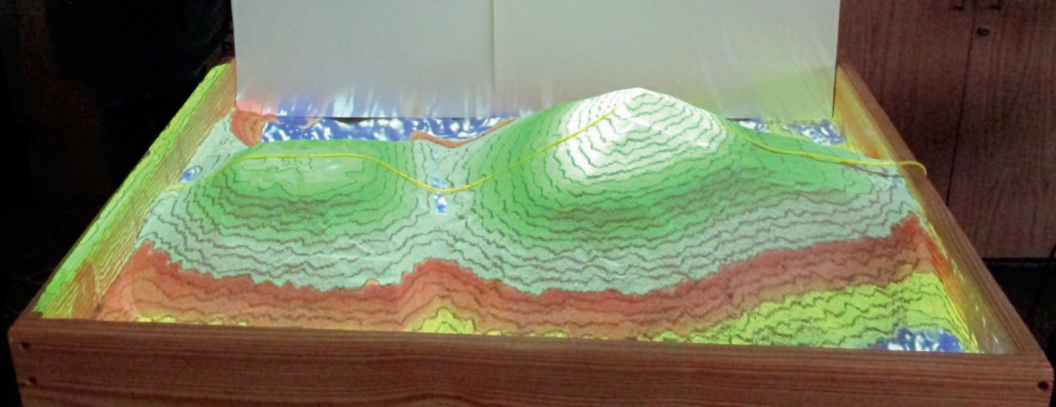
\includegraphics[width=0.9\linewidth]{figure/Analysis/augmentedrealitysandbox.png}
		\caption{Augmented reality sandbox showing a topographical map of the sand. Simulated water can be seen on the other side of the hill \cite{woods2016pilot}.}
		\label{fig:augmentedrealitysandbox}
	\end{figure}



\subsection{Leap Motion} % Daniel
    Leap motion is a tool that is used for tracking hands and fingers in real time\cite{leapMotion}. The newest iteration integrates with Virtual Reality, hence eliminating the need for having a controller in your hand. The Leap Motion controller functions by having three IR LEDs and two monochromatic IR Cameras. The maximum reading distance from the controller is approximately 1m\cite{leapMotion}. The accuracy of the controller is roughly 0.7mm, hence the virtual version of ones hands can be very precise as seen in \autoref{fig:leapMotion}.
    
    \begin{figure}[H]
    	\centering
    	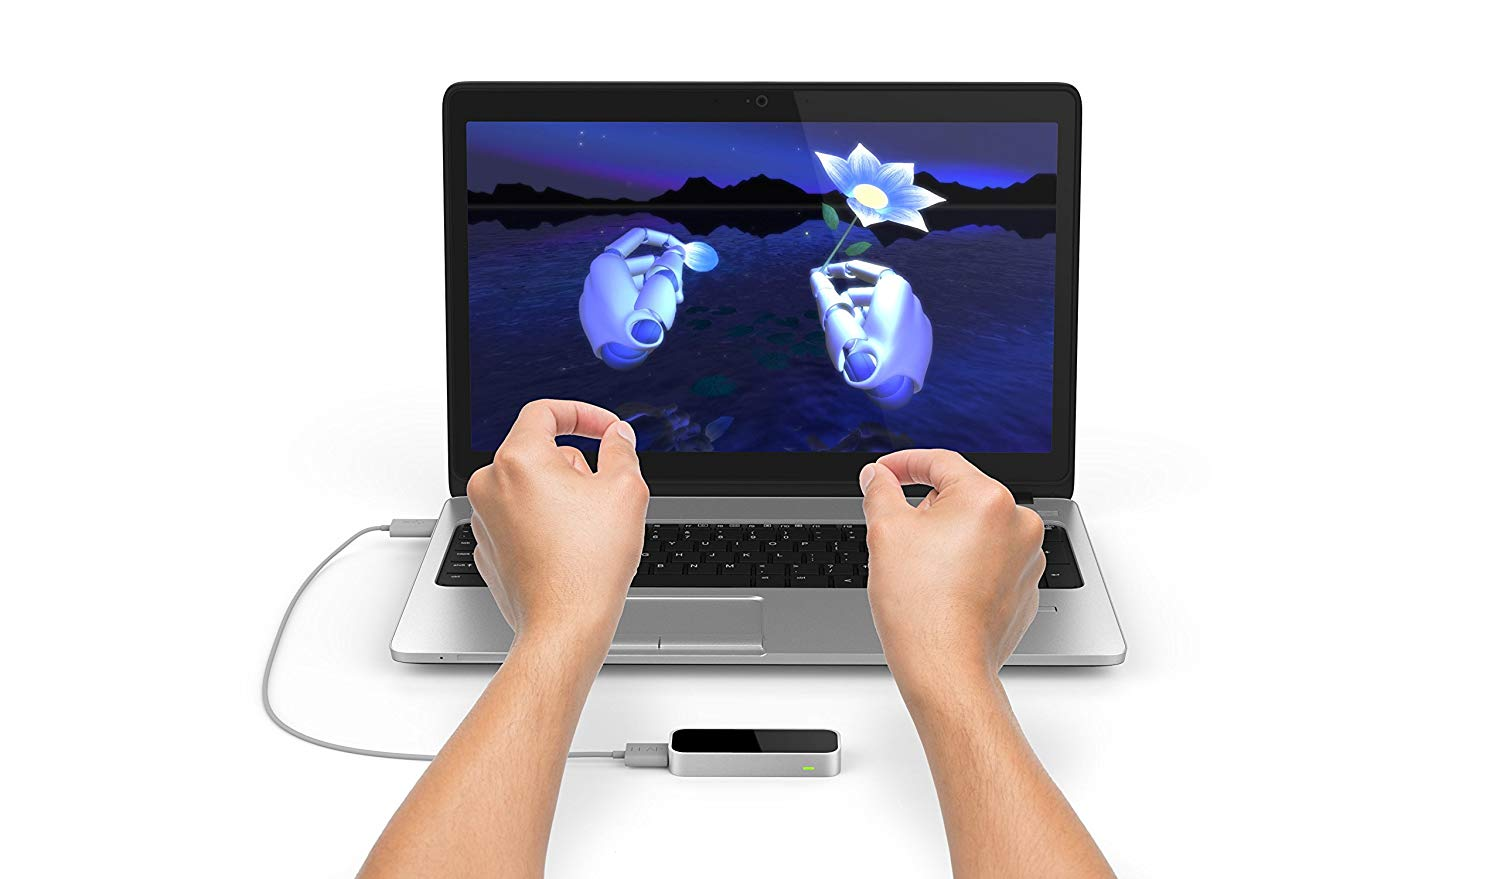
\includegraphics[width=0.9\linewidth]{figure/Analysis/leapMotion.jpg}
    	\caption{Image of the Leap Motion in action, taken from the Amazon store page.}
    	\label{fig:leapMotion}
    \end{figure}
    
\subsection{Immersive Holodeck}\label{sec:leapMotionHolodeck} % Daniel
    A university in Ohio made an immersive \textit{"holodeck"} like experience, using 3 projectors in combination with a Leap Motion positioned in the the middle of the room. Using the leap motion, a user could manipulate objects in minecraft, like seen in \autoref{fig:holodeck}, or navigate around the world using Google maps\cite{leapMotionHolodeck}.
    
    \begin{figure}[H]
    	\centering
    	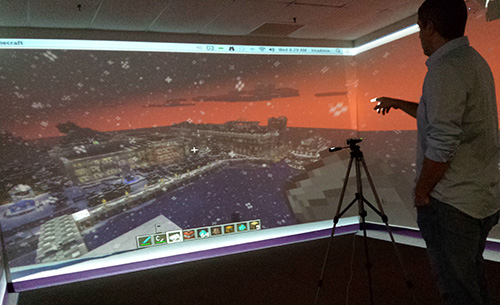
\includegraphics[width=0.7\linewidth]{figure/Analysis/holodeck.jpg}
    	\caption{Ohio university made immersive holodeck, made for immersive language learning\cite{leapMotionHolodeck}.}
    	\label{fig:holodeck}
    \end{figure}
    
    The purpose of the system, was to allow immersion while learning a language, putting you in the environments that the language is spoken.
    
    	\subsection{Interactive Projection Mapping Prototype} % Daniel
	    This project demonstrates the possibilities of manipulating the physical world using the Leap Motion in combination with an Arduino, as seen in \autoref{fig:leapProjector}. Using the Leap Motion API \todo{as described in section XYZ}, the creator allowed for simple gestures to control the box and pick up the pets in the world. The goal of the game is as simple as picking up the four pets and putting them on their pillow, all while rotating the cube to cycle through the different seasons and sides of the cube\cite{leapMotionProjectionMapping}.
	    \begin{figure}[H]
	    	\centering
	    	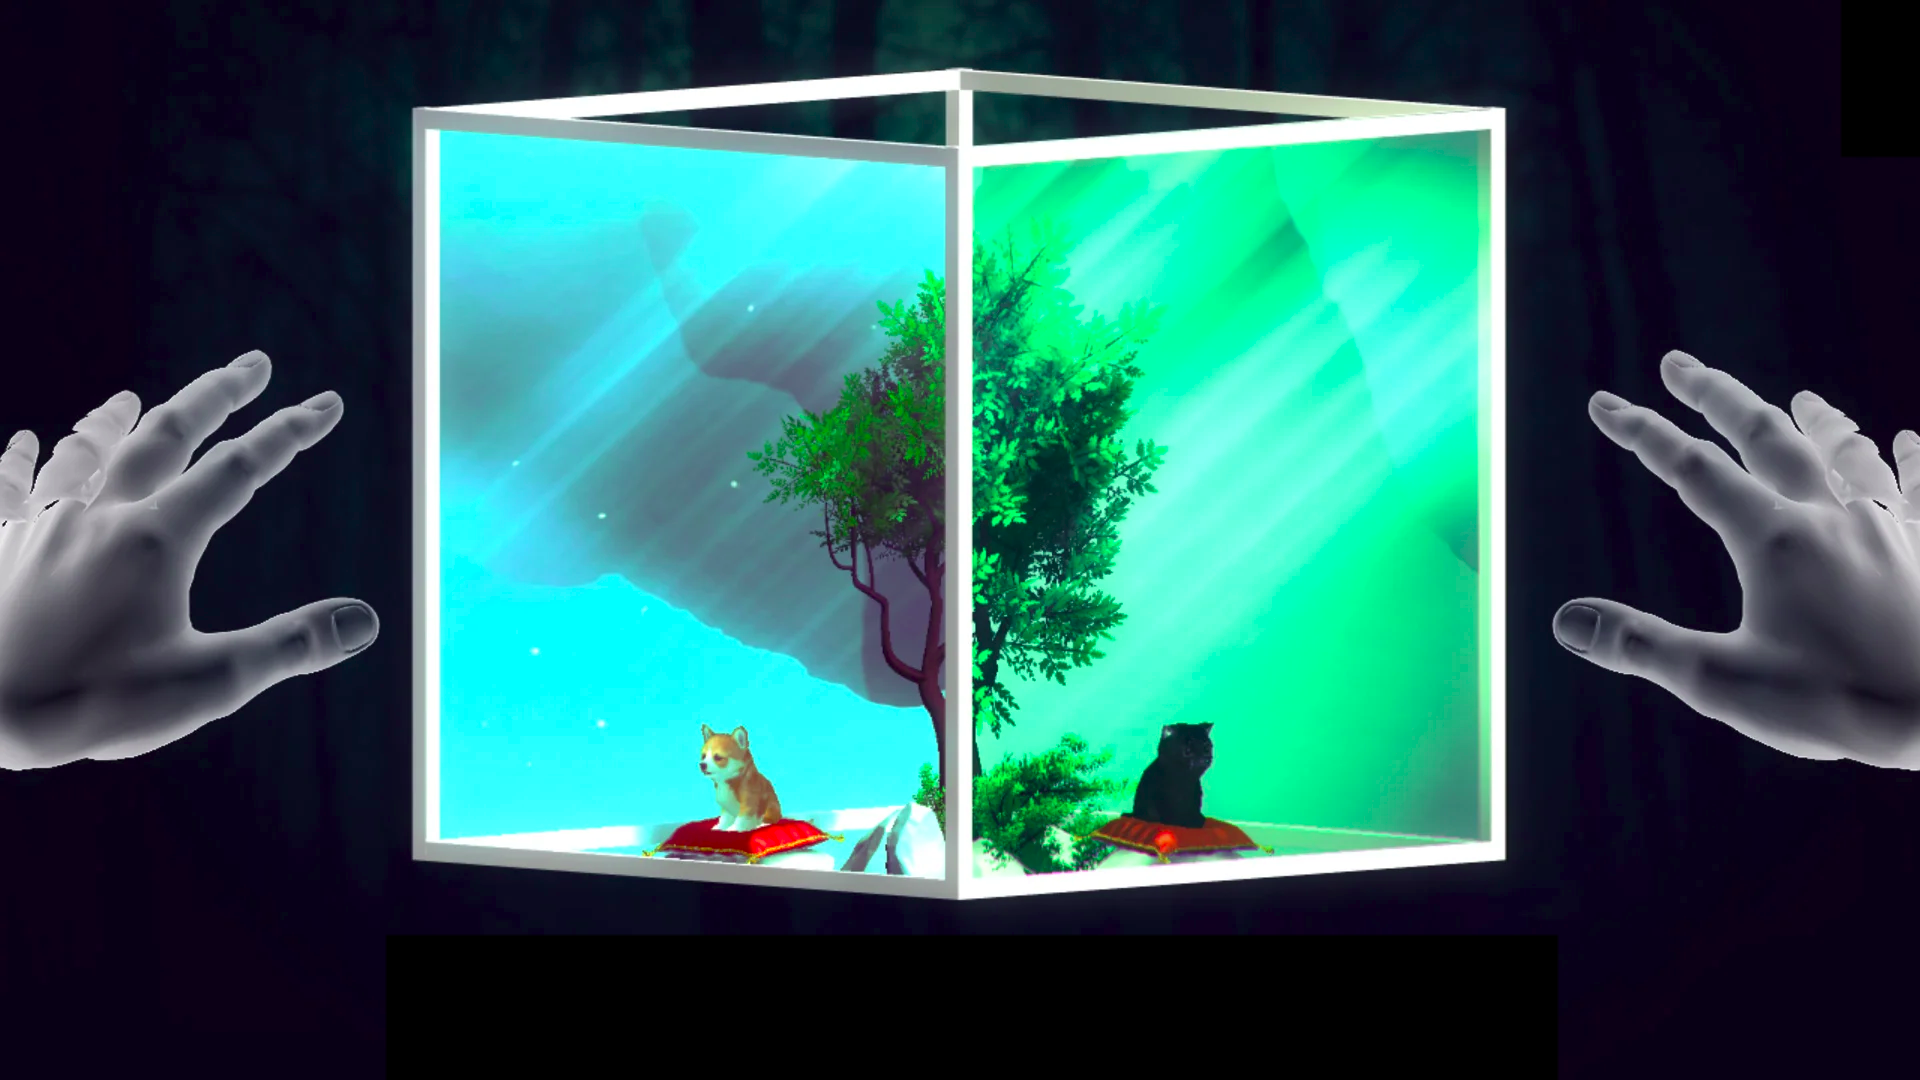
\includegraphics[width=0.8\linewidth]{figure/Analysis/LeapProjector.png}
	    	\caption{A physical game, using the Leap Motion to pick up pets and rotating the physical cube using gestures\cite{leapMotionProjectionMapping}.}
	    	\label{fig:leapProjector}
	    \end{figure}
    The game can be played exclusively on the PC, without the physical cube. But the point from the creator's side was to learn to interface with the physical cube using the Leap Motion.


\subsection{Multiple Display setups}
As seen in \autoref{sec:leapMotionHolodeck} and \autoref{sec:transcendingBoundaries} multiple projectors working in tandem are utilized to create immersive technology. There are several ways of having multiple projectors working together. Using a Graphical Processing Unit, or GPU for short with sufficient outputs to drive all the required projectors. Newer graphics cards can run up to 4 monitors at the same time \footnote{GTX 1080TI: \url{https://www.evga.com/products/product.aspx?pn=11G-P4-6693-K3}}, or with the use of a display port hub, splitting the bandwidth of the display ports to allow more monitors at lower resolutions\footnote{EVGA DisplayPort Hub\url{https://www.evga.com/products/product.aspx?pn=200-dp-1301-l1}} which makes it possible to run even more screens off a single high end GPU, depending on how many display ports it has. If more monitors than this are needed, multiple GPU's can be installed in the same system, and even more displays can be used. Another way to achieve multiple displays with a single display port is using a technology called daisy chaining. The principle behind this is to connect multiple displays supporting display ports where each one is connected in sequence to each other, hence only requiring one output from the GPU. Depending on the resolution this can be done with 2-5 monitors\cite{displayport}.

\subsection{Interactive display at "The Blue Planet"}
The Blue Planet is an aquarium located in Copenhagen, Denmark. It's a new and modern facility, with several digital interactive installations. One installation is designed to make the users be the current of the ocean. Projectors show micro organisms on a wall and a Microsoft Kinect detects movement from users. As users walk by the wall, the shadow of the users pushes the micro organisms away from themselves, making the display behave according to the movement of the users.\cite{DenBlaPlanet} 

\subsection{Transcending Boundaries}\label{sec:transcendingBoundaries} % Jens
Transcending Boundaries is an exhibition that ran in the beginning of 2017 at the Pace Gallery in London. It featured a series of immersive installations made by teamLab in an attempt to transcend the boundaries between digital artwork and the physical world\cite{transcendingBoundries}. \autoref{fig:transcendingBoundaries} shows a virtual waterfall, flowers and butterflies that are projected up on the walls and on the floor in one of the rooms of the exhibit using multiple projectors. The vegetation would indicate changes in seasons and would go through all 4 seasons every hour. Viewers in the room would obstruct the flow of water based on where they were standing and thereby became a part of the artwork. 

    \begin{figure}[H]
    	\centering
    	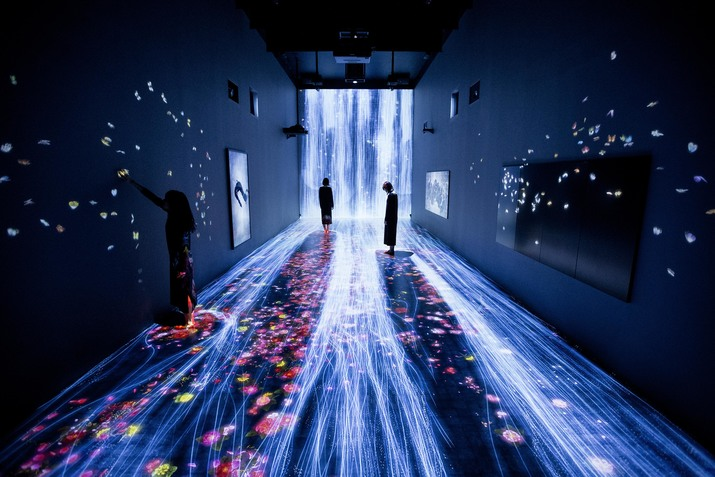
\includegraphics[width=0.9\linewidth]{figure/Analysis/transcendingBoundaries.jpg}
    	\caption{Figure showing 3 people interacting with the virtual waterfall installation from teamLab's exhibition at the Pace Gallery in London\cite{transcendingBoundries}.}
    	\label{fig:transcendingBoundaries}
    \end{figure}
    
